
\section{Implementation}
\label{sec:Implementation}

\subsection{Komponenten}
\label{impl:Komponenten}

\subsection{PlazaRoute Container}
\label{impl:PlazaRoute Container}
TODO

\subsubsection{Plaza Vorverarbeitung}
\label{impl:Plaza Vorverarbeitung}

In diesem Kapitel wird die Umsetzung der Plaza Vorverarbeitung, wie sie in Kapitel \ref{architektur:Plaza Vorverarbeitung} beschrieben ist, erläutert. Dabei wird das Zusammenspiel der verschiedenen Komponenten aufgezeigt und einige Implementationsdetails diskutiert.

Die Code-Dokumentation der Plaza Vorverarbeitung ist unter \cite{PlazaRoute-apidoc} veröffentlicht.

\paragraph{Struktur und Ablauf der Komponenten} \label{impl:Struktur der Komponenten} ~\\
Die Python-Pakete wurden anhand der Architektur und des Datenflusses, wie in Abbildung \ref{fig:dataflow_vorverarbeitung} zu sehen, strukturiert. So wurde für jede Komponente \emph{OSM Importer}, \emph{Plaza Optimizer} und \emph{OSM Merger} ein eigenes Python-Subpackage erstellt.

Angestossen wird die Vorverarbeitung vom \code{\_\_main\_\_.py} file, das vom Benutzer mit der Kommandozeile aufgerufen wird.

\begin{figure}[ht]
    \centering
    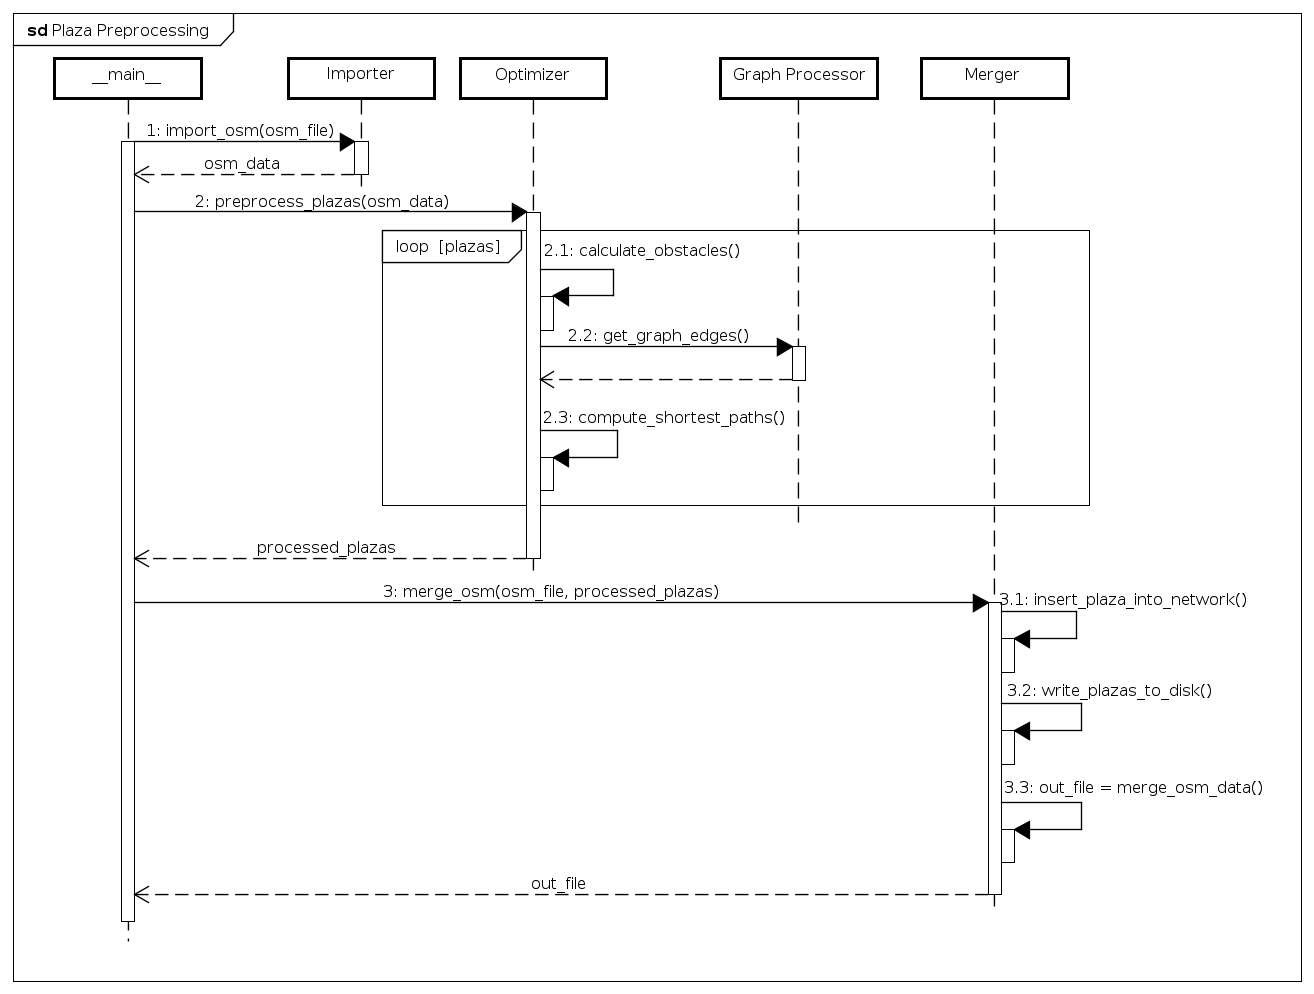
\includegraphics[width=1\linewidth]{projectdoc/img/sequence_diagram_plaza_preprocessing.png}
    \caption[Sequenz Diagramm Plaza Vorverarbeitung]{Sequenz Diagramm Plaza Vorverarbeitung}
    \label{fig:sequence_diagram_plaza_preprocessing}
\end{figure}

In Abbildung \ref{fig:sequence_diagram_plaza_preprocessing} ist der Ablauf in einem Sequenzdiagramm dargestellt. Dies entspricht nicht komplett dem Programmcode, sondern soll nur zur Veranschaulichung des Zusammenspiels der einzelnen Komponenten dienen.

Im Folgenden wird auf die einzelnen Komponenten eingegangen.

\paragraph{Importer}\label{impl:Importer}~\\
Das Importer-Package liest aus einer gegebenen \ac{OSM}-Datei (Dateityp \ac{OSM} oder \ac{PBF}) die für uns relevanten Daten mit Hilfe von Pyosmium \cite{pyosmium} ein. Während dem Einlesen werden die benötigten Daten direkt heraus gefiltert. Für uns relevant sind vor allem Plazas, die anhand von konfigurierbaren Tags bestimmt werden. Zusätzlich werden alle Strassen benötigt, um die Plazas später wieder an das Strassennetz anzuschliessen (siehe Abschnitt \nameref{impl:Merger}). Punkte und Gebäude werden für die Berechnung von Hindernissen auf den Plazas genutzt.

Alle ausgelesenen Daten werden in ein \code{OSMHolder} Objekt verpackt und zurück gegeben.

\paragraph{Optimizer}\label{impl:Optimizer}~\\
Der Optimizer übernimmt die Kernfunktion der Vorverarbeitung, die Optimierung von Fussgänger-Flächen.

Das \code{OSMHolder}-Objekt aus dem \nameref{impl:Importer} wird de Optimizer übergeben. Als erstes wird für Strassen, Punkte und Gebäude je ein R-Tree \cite{rtree_Guttman} Index erstellt. Dies erlaubt es uns, effizient geometrische Objekte zu finden, die sich mit dem Plaza schneiden. Ohne einen Index müsste für jedes Objekt (Linie, Punkt oder Gebäude) jeweils der komplette Datensatz durchsucht werden ($O(n)$). Mit einer Index-Suche ($O(\log n)$) werden die Datensätze auf ein paar wenige mögliche Treffer eingegrenzt.

Für jedes Plaza werden folgende Schritte ausgeführt:
\begin{enumerate}
    \item Es werden alle \glspl{Einstiegspunkt} berechnet. Plazas, die weniger als zwei Einstiegspunkte haben, werden direkt verworfen, da auf diesen mit unserem Algorithmus gar keine kürzesten Wege berechnet werden könnten.
    \item Linien, die das Plaza schneiden und einen \gls{Einstiegspunkt} bilden, werden mit der \ac{OSM} ID zwischengespeichert. Die jeweiligen \glspl{Einstiegspunkt} werden später vom \nameref{impl:Merger} in diese Linien eingefügt.
    \item Alle Hindernisse auf dem Plaza werden ausgeschnitten. Dies kann ein Gebäude sein, das auf dem Platz steht, oder ein Hindernis wie z.B. ein Brunnen. Solche Hindernisse werden mit einem Quadrat mit konfigurierbaren Radius ausgeschnitten. Sollte nach diesem Schritt das Plaza komplett von Gebäuden oder Hindernissen verdeckt sein, wird es verworfen.
    \item Nun findet die eigentliche Optimierung statt, das Berechnen eines Graphen über das Plaza. Als Knotenpunkte des Graphen werden die \glspl{Einstiegspunkt} sowie alle Eckpunkte des Polygons (dementsprechend auch von Hindernissen) beachtet. Es sind die beiden Verfahren SpiderWeb Graph und Visibility Graph implementiert. Das Verfahren kann über das Strategy-Pattern \cite{gof_patterns} konfiguriert werden.
    \item Um die Anzahl Kanten des Graphen zu verringern, werden aus den generierten Graphen alle kürzesten Wege von jedem Einstiegspunkt zu jedem anderen Einstiegspunkt berechnet. Dies kann mit dem Dijkstra- \cite{dijkstra_algorithm} oder A*-Algorithmus \cite{astar} durchgeführt werden. Alle Kanten, die nicht auf diesen kürzesten Pfade sind, werden verworfen.
    \item Für den SpiderWeb Graphen wird zusätzlich die Anzahl Knotenpunkte in den kürzesten Pfaden reduziert, indem die Linien geglättet werden. Dazu wird mit Hilfe von Shapely \cite{shapely} der Douglas-Peucker Algorithmus \cite{douglas-peucker_algorithm} verwendet.
\end{enumerate}


\paragraph{Merger}\label{impl:Merger}~\\
Die Aufgabe des Merger ist es, die vom \nameref{impl:Optimizer} neu erstellten Geometrien wieder mit den originalen \ac{OSM}-Daten zu verschmelzen.
\begin{enumerate}
    \item In einem ersten Schritt werden die erstellten Linien im \ac{OSM}-Format als Nodes und Ways in eine temporäre Datei gespeichert.
    \item Als nächstes werden die Einstiegspunkte in das Strassennetz eingebunden. Nur wenn unsere Linien einen gemeinsamen Punkt mit dem bestehenden Strassennetz haben, werden sie vom Router überhaupt für das Routing beachtet. Da sich jeder Einstiegspunkt mit einer bestehenden Linie kreuzt, wird dieser jeweils als zusätzlicher Punkt dem \ac{OSM}-Way hinzugefügt.
    \item Die im vorherigen Schritt modifizierten Ways werden ebenfalls in eine temporäre Datei abgespeichert. Dazu wird die Versionsnummer erhöht, damit die bestehenden Ways schlussendlich überschrieben werden.
    \item Nun werden alle in den vorherigen Schritten erstellten temporären \ac{OSM}-Dateien mit der originalen Datei zusammen geschmolzen, die ursprünglich importiert wurde. Dazu wird das externe Tool Osmosis \cite{osmosis} aufgerufen.
\end{enumerate}

Als Endresultat liegt nun eine \ac{OSM}-Datei mit den kompletten Kartendaten vor, die um zusätzliche Linien für die Optimierung über Fussgängerflächen ergänzt wurde. Die Datei kann nun etwa einer Routing-Engine übergeben werden.

\subsubsection{Plaza Routing}
\label{impl:Plaza Routing}
In den folgenden Unterkapitel wird die Umsetzung der Plaza Routing Architektur, welche im Kapitel \ref{architektur:Plaza Routing} definiert ist, erläutert. Dabei handelt es sich um eine Flask-Applikation\cite{flask}.

\paragraph{app}\label{impl:app-layer}~\\
Die Flask-Applikation\cite{flask} wird in dieser Komponente konfiguriert und gestartet. So wird unter anderem das Logging aufgesetzt und die \ac{API}, welche im Abschnitt \nameref{impl:Plaza Routing api} beschrieben ist, initialisiert.

Ebenfalls werden hier Error-Handler definiert, welche dafür sorgen, dass der Konsument der \ac{API} eine ansprechende und informative Fehlermeldung erhält und sicherstellt, dass keine Implementationsdetails der Applikation exponiert werden.

\paragraph{api}\label{impl:Plaza Routing api}~\\
In diesem Abschnitt wird auf die Umsetzung der api-Schicht in Abbildung \ref{fig:package_diagram_plaza_routing} und auf den Abschnitt \nameref{architektur:api-layer} in der Architektur Bezug genommen.

Dabei wird mithilfe von Flask-RESTPlus \cite{flask-restplus}, einer Flask-Extension, eine \ac{REST}-\ac{API} exponiert. Diese besteht aktuell aus einem \ac{REST}-Service, welcher im Abschnitt \nameref{impl:PlazaRouting} genauer erläutert ist. Die Extension hat den Vorteil, dass automatisch eine Swagger-Dokumentation \cite{swagger} generiert wird, mit welcher unter anderem \ac{API}-Clients in verschiedenen Programmiersprachen generiert werden können. Diese ist unter \cite{plaza-routing-api-swaggerui} verfügbar. Ebenfalls ist sofort ersichtlich, wie das Response-Model der \ac{API} aussieht und in welchem Format, welche Parameter übergeben werden müssen. Dies Vereinfacht die Handhabung mit der \ac{API} massiv.

Diese Komponenten kann ohne Probleme mit \ac{REST}-Services analog zu \nameref{impl:PlazaRouting} ergänzt werden.

\subparagraph{PlazaRouting}\label{impl:PlazaRouting}~\\
In der Komponenten \emph{PlazaRouting} wird der \ac{REST}-Service für das Routing exponiert. Im Bezug auf das Maturity Model \cite{maturity_model} von Leonard Richardson befinden wir uns auf Level 2. Im \ac{REST}-Service werden die übergebenen Parameter entgegen genommen, automatisch in das verlangte Format geparsed und geprüft, ob die Parameter, welche zwingend verlangt werden, auch übergeben wurden. Diese Information wird dann weiter an die Business-Schicht gereicht, welche im nächsten Abschnitt aufgeschlüsselt wird. Die Komponente besitzt sonst keine weitere Logik.

\paragraph{Zusammenspiel und Verantwortlichkeit der Business- und Service-Schicht}\label{impl:Plaza Routing Zusammenspielund Verantwortlichkeit der Business- und Service-Schicht}~\\
In Abbildung \ref{fig:sequence_diagram_plaza_routing_overview} sind die Interaktionen zwischen den Komponenten in einem Sequenz-Diagramm aufgeschlüsselt. Dabei wurde zur Wahrung der Übersichtlichkeit das Holen aller möglichen Routen und das Optimieren der besten Route in ein Unter-Sequenz-Diagram in Abbildung \ref{fig:sequence_diagram_plaza_routing_route_combs}, respektive Abbildung \ref{fig:sequence_diagram_plaza_routing_optimize_route_comb} ausgelagert. Dabei geht es primär nicht um die Logik, die dahinter liegt, sondern um die Verantwortlichkeiten der Services. Wann sie ins Spiel kommen und für was sie benötigt werden, ist so gut ersichtlich. Aus diesem Grund entsprechen die Diagramme nicht exakt dem Programmcode. 

Die Ausgangsposition und Destination können entweder als Koordinate oder Adresse übergeben werden. Falls es sich um eine Adresse handelt, wird ein Geocoding durchgeführt, um die Koordinate zu extrahieren. Dies erklärt den zweimaligen Zugriff auf das \emph{Geocoding} im Sequenz-Diagramm \ref{fig:sequence_diagram_plaza_routing_overview}.

\begin{figure}[ht]
    \centering
    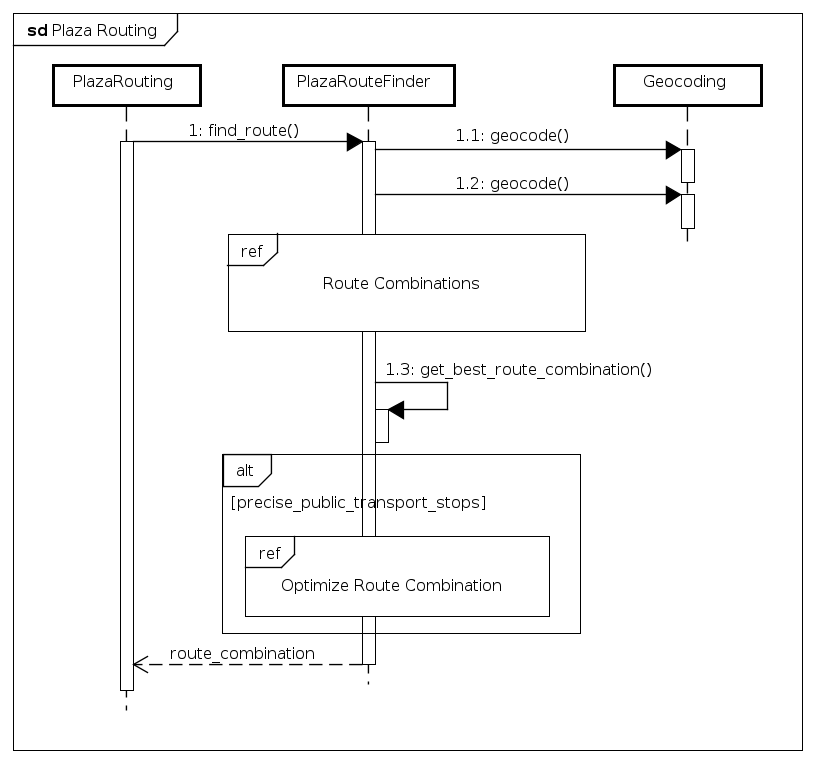
\includegraphics[width=0.7\linewidth]{projectdoc/img/sequence_diagram_plaza_routing_overview}
    \caption[Plaza Routing Sequenz-Diagramm Übersicht]{Plaza Routing Sequenz-Diagramm Übersicht}
    \label{fig:sequence_diagram_plaza_routing_overview}
\end{figure}

\begin{figure}[ht]
    \centering
    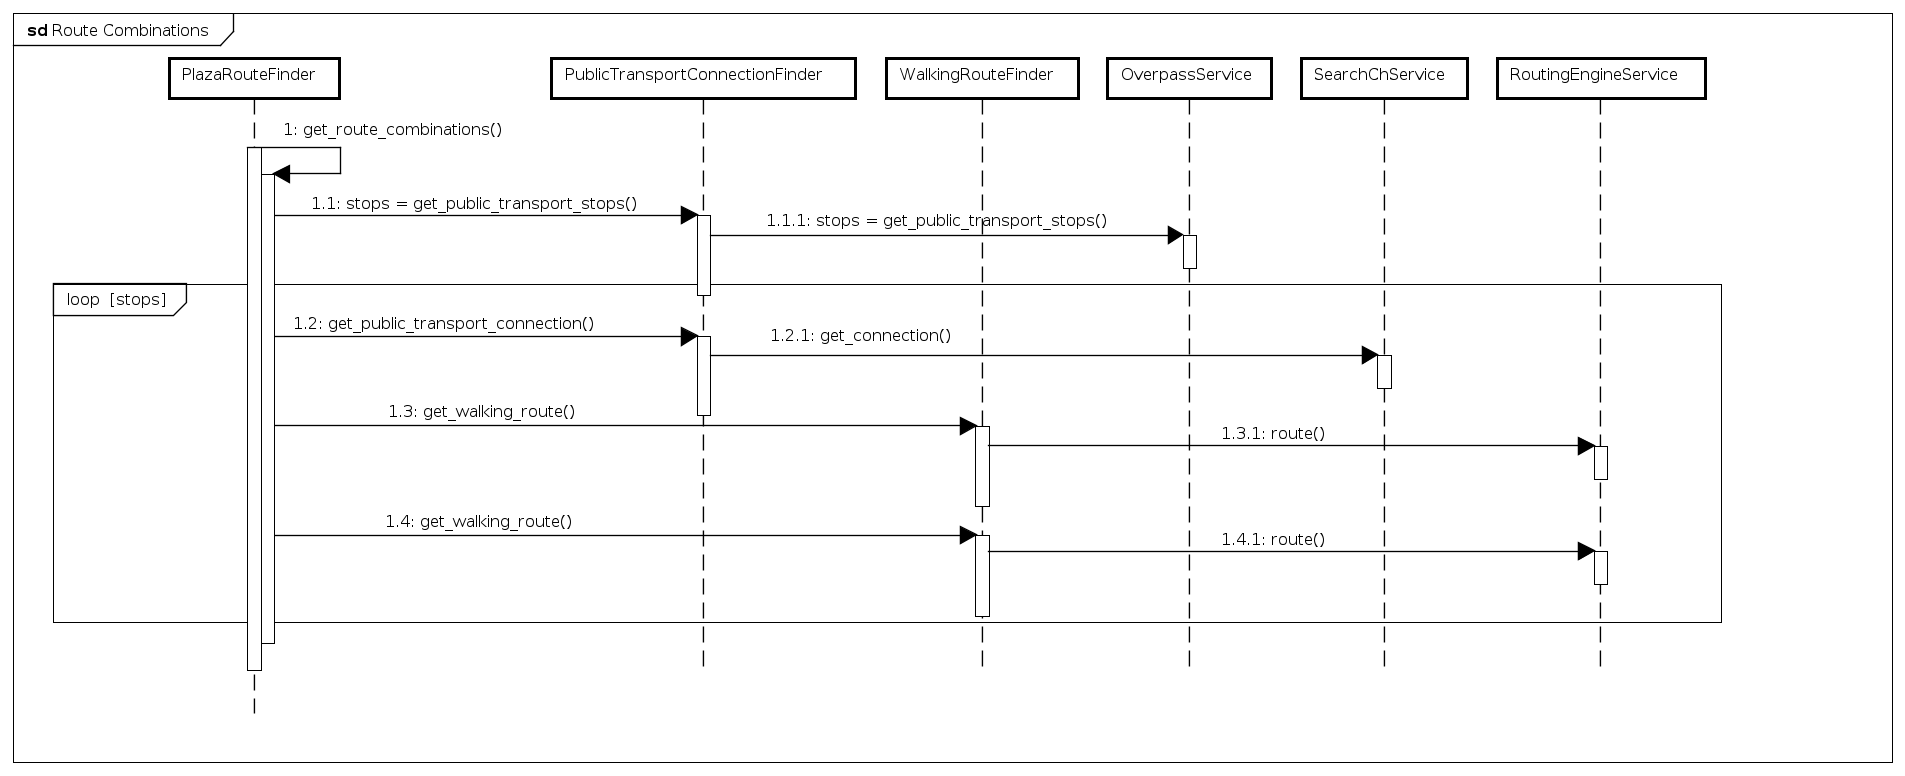
\includegraphics[width=1\linewidth]{projectdoc/img/sequence_diagram_plaza_routing_route_comb}
    \caption[Plaza Routing Sequenz-Diagramm Route Combinations]{Plaza Routing Sequenz-Diagramm Route Combinations}
    \label{fig:sequence_diagram_plaza_routing_route_combs}
\end{figure}

Man sieht in Abbildung \ref{fig:sequence_diagram_plaza_routing_route_combs} gut, dass im Loop für eine Ausgangs-ÖV-Station die Verbindung von search.ch \cite{search_ch_route_api} geholt (siehe Abschnitt \nameref{impl:Plaza Routing ÖV-Haltestellen eruieren}) und zwei Mal eine Fussgänger-Routing durchgeführt wird, jeweils vom aktuellen Standort zur ersten ÖV-Station und von der letzten ÖV-Station zur Destination. Diese Daten sind die Grundlagen für die Entscheidungsfindung der besten Route, welche in Abschnitt \nameref{impl:Plaza Routing Beste Route eruieren} beschrieben ist. \emph{Optimize Route Combination} ist im Abschnitt \nameref{impl:Plaza Routing Route optimieren} genauer beschrieben.

\paragraph{ÖV-Haltestellen eruieren}\label{impl:Plaza Routing ÖV-Haltestellen eruieren}~\\
ÖV-Haltestellen werden mit Overpass \cite{wiki:overpass} aus \ac{OSM} bezogen. Dabei wird um den aktuellen Standort eine \gls{BoundingBox} gezogen. Die Bounding Box ist konfigurierbar und entspricht einer zumutbaren Laufdistanz. In dieser Fläche werden Nodes und Relationen mit Tags, welche ÖV-Haltestellen identifizieren (\emph{''public\_transport''=''stop\_position''}, \emph{''type''=''public\_transport''} etc.), gefiltert und deren \emph{uic\_ref} zurückgegeben.

\paragraph{Beste Route eruieren}\label{impl:Plaza Routing Beste Route eruieren}~\\
% TODO was machen wir eigentlich, wenn zwei Verbindungen die gleichen Kosten haben?
Aufgrund der möglichen Routen, welche wie in Abbildung \ref{fig:sequence_diagram_plaza_routing_route_combs} gewonnen werden, muss man nun entscheiden, welche Route dem User konkret retourniert wird. Dazu wurde eine Kosten-Matrix erstellt. Diese ist in Tabelle \ref{table:cost-matrix} sichtbar.

\begin{table}[ht]
    \centering
    \begin{tabular}{l|l}
        & \textbf{Gewicht} \\ \hline
        \textbf{Gehzeit}                    & 2                \\
        \textbf{Dauer der ÖV-Verbindung}    & 1                \\
        \textbf{Anzahl der ÖV-Teilstrecken} & 7 * 60          
    \end{tabular}
    \caption{Kosten-Matrix}
    \label{table:cost-matrix}
\end{table}

Die Dauer des Fussstrecke wird doppelt gewichtet. Ein einmaliges Umsteigen schlägt mit 7 Minuten ins Gewicht. So lassen sich die Kosten aufgrund der Zeit, welche man für jeden Faktor benötigt, berechnen.

Eine Verbindung, bei welcher man 5 Minuten geht, 15 Minuten fährt und zwei Mal umsteigen muss, wird mit Totalkosten von $5 * 60 * 2 + 15 * 60 + 2 * 7 * 60 = 2340$ mit den anderen möglichen Verbindungen verglichen. Schlussendlich wird die Verbindung mit den niedrigsten Kosten retourniert.

\paragraph{Route optimieren}\label{impl:Plaza Routing Route optimieren}~\\
Search.ch \cite{search_ch_route_api} liefert in einer ÖV-Verbindung für zwei gegenüberliegenden Haltestelle (je eine für jede Fahrrichtung) eine Koordinate zurück, welche beispielsweise direkt auf der Hauptstrasse liegen kann (siehe Abbildung \ref{fig:one_coordinate_for_two_stops}). Dies ist für ein Fussgänger-Routing suboptimal.

\begin{figure}[ht]
\centering
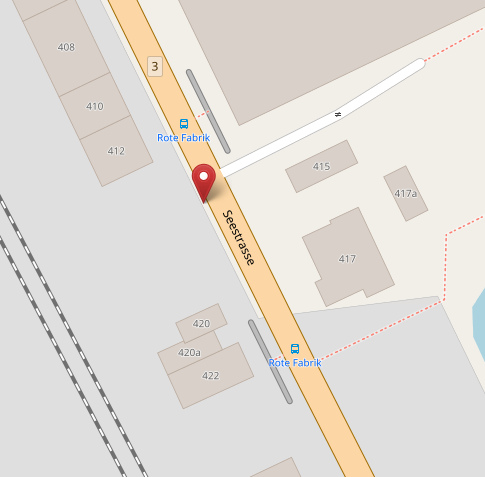
\includegraphics[width=0.5\linewidth]{projectdoc/img/one_coordinate_for_two_stops}
\caption[eine Koordinate für zwei ÖV-Stationen]{eine Koordinate für zwei ÖV-Stationen der Roten Fabrik, Zürich, Schweiz; openstreetmap.org; Screenshots aufgenommen am 25.11.2017}
\label{fig:one_coordinate_for_two_stops}
\end{figure}

Aus diesem Grund werden diese Koordinaten nun von Overpass \cite{wiki:overpass} bezogen. Der Ablauf ist schematisch in Abbildung \ref{fig:sequence_diagram_plaza_routing_optimize_route_comb} dargestellt. So wird für jede ÖV-Teilstrecke die Koordinate für die Einstieg- und Ausstiegsstation geladen. Nach dem Laden muss nochmals das Fussgänger-Routing durchgeführt werden, da sich die Koordinate der ersten und letzten ÖV-Station verändert haben.

\begin{figure}[ht]
\centering
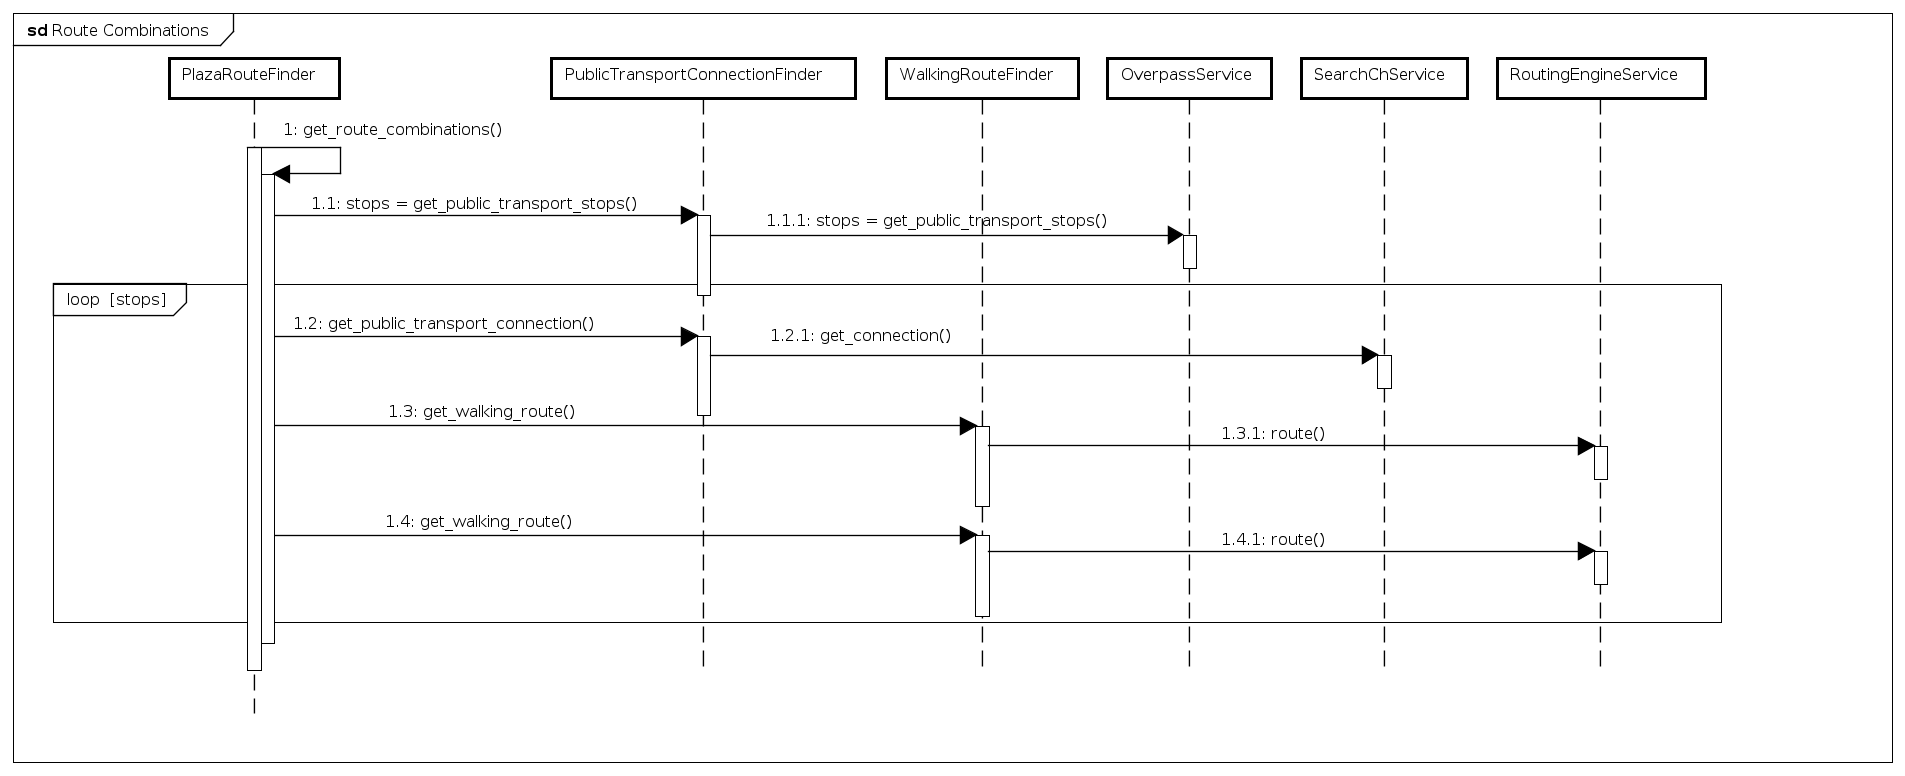
\includegraphics[width=1\linewidth]{projectdoc/img/sequence_diagram_plaza_routing_optimize_route_comb}
\caption[Plaza Routing Sequenz-Diagramm Optimize Route Combination]{Plaza Routing Sequenz-Diagramm Optimize Route Combination}
\label{fig:sequence_diagram_plaza_routing_optimize_route_comb}
\end{figure}

Da ÖV-Stationen und -Linien in \ac{OSM} jedoch nicht konsistent gemappt sind, wird das Recovery Blocks Pattern \cite{fault_tolerant_software} angewendet, um dem User so oft wie möglich ein genaues Resultat liefern zu können. Mit nicht konsistent meinen wir, dass sie nicht zwingend den Vorgaben in \cite{osm_wiki_relation} folgen. Durch Tests lassen sich jedoch Trends erkennen, wie Mapper grundsätzlich mit ÖV-Verbindungen umgehen.

Vorgängig muss klargestellt werden, dass wenn die Rede vo einer Linie ist, grundsätzliche eine Buslinie oder ähnliches, welches in \ac{OSM} als Relation \cite{osm_wiki_relation} abgebildet ist, gemeint ist. Spricht man von einer Station, ist die ÖV-Station gemeint, welche als Node gemappt ist.

In einem ersten Schritt werden die Daten über die bekannte ÖV-Linie geladen. Search.ch \cite{search_ch_route_api} liefert eine \emph{uic\_ref} für die initiale ÖV-Station und eine bei welcher man aussteigt. Üblicherweise erhält man zwei Relationen zurück, je eine für jede Fahrrichtung. Mit den beiden Stationen kann man nun die Members der Relation durchgehen und die Linie selektieren, bei welcher die \emph{uic\_ref} der initialen ÖV-Station vor der \emph{uic\_ref} der Ausstiegsstation kommt.
Anmerken muss man, dass es natürlich mit einem Risiko verbunden ist, so die korrekte Koordinate zu eruieren. Entspricht die Reihenfolge der Members nicht der tatsächlichen Reihenfolge der ÖV-Stationen, kommt aber bei beiden Relationen oder der Falschen die \emph{uic\_ref} der initialen ÖV-Station vor der \emph{uic\_ref} der Ausstiegsstation, kann es vorkommen, dass man die falsche Station erwischt. Mit diesem Restrisiko leben wir.

Ist die erste Variante nicht erfolgreich, werden die Relationen mit der \emph{uic\_ref} der initialen ÖV-Station geladen. ÖV-Stationen mit der gleichen \emph{uic\_ref} gehören normalerweise zu einer Relation, welche auch selbst diese \emph{uic\_ref} besitzt. Über diese Relation können die möglichen initialen Ausgangsstationen und die Linien geladen werden. In einem weiteren Schritt werden die Ausstiegstationen in einem ähnlichen Verfahren für die \emph{uic\_ref} der Ausstiegsstation geladen. Im idealen Fall hat man nun die Einstiegsstationen, Linien und Ausstiegstationen für beide Fahrtrichtungen. Mit diesen Daten kann nun die korrekte Einstiegs- und Ausstiegstation der konkreten Linie zugeordnet werden (durch ihre Zugehörigkeit als Member). Da man die Einstiegs- und Ausstiegstation separat geladen hat, ist es eine Leichtigkeit, die Linie in die richtige Fahrtrichtung zu eruieren.

Führen diese zwei Varianten nicht zum Ziel, wird die Koordinate von search.ch zurückgegeben.

Das Verbesserte Resultat von Abbildung \ref{fig:one_coordinate_for_two_stops} ist in Abbildung \ref{fig:one_coordinate_for_two_stops_improved} ersichtlich.

\begin{figure}[ht]
    \centering
    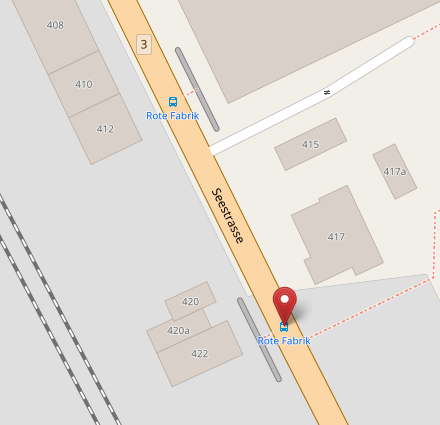
\includegraphics[width=0.5\linewidth]{projectdoc/img/one_coordinate_for_two_stops_improved}
    \caption[mit Overpass geladenen Koordinate]{mit Overpass geladenen Koordinate der Roten Fabrik in Richtung Seerose, Zürich, Schweiz; openstreetmap.org; Screenshots aufgenommen am 25.11.2017}
    \label{fig:one_coordinate_for_two_stops_improved}
\end{figure}


Die erhöhte Genauigkeit kommt nicht ohne Performanzeinbusse. Im Worst-Case wird drei Mal eine Overpass-Abfrage \cite{wiki:overpass} für jede ÖV-Teilstrecke durchgeführt und schlussendlich doch die Fallback-Koordinate von search.ch \cite{search_ch_route_api} retourniert. Aus diesem Grund kann man beim Aufruf des \ac{REST}-Service ein optionales Flag setzen, welches dem User die Antwort auf die Frage überlässt, ob er diese Genauigkeit will oder mit der Koordinate von search.ch \cite{search_ch_route_api} zufrieden ist. Bei gesetztem Flag beschränken sich die Zugriffe auf Overpass \cite{wiki:overpass} auf das Holen der ÖV-Haltestellen.

\subsection{QGIS Plugin}
\label{impl:QGIS Plugin}
TODO
